% To je predloga za poročila o domačih nalogah pri predmetih, katerih
% nosilec je Blaž Zupan. Seveda lahko tudi dodaš kakšen nov, zanimiv
% in uporaben element, ki ga v tej predlogi (še) ni. Več o LaTeX-u izveš na
% spletu, na primer na http://tobi.oetiker.ch/lshort/lshort.pdf.
%
% To predlogo lahko spremeniš v PDF dokument s pomočjo programa
% pdflatex, ki je del standardne instalacije LaTeX programov.

\documentclass[a4paper,11pt]{article}
\usepackage{enumitem}
\usepackage{a4wide}
\usepackage{fullpage}
\usepackage[utf8x]{inputenc}
\usepackage[slovene]{babel}
\selectlanguage{slovene}
\usepackage[toc,page]{appendix}
\usepackage[pdftex]{graphicx} % za slike
\usepackage{setspace}
\usepackage{color}
\definecolor{light-gray}{gray}{0.95}
\usepackage{listings} % za vključevanje kode
\usepackage{hyperref}
\usepackage{subcaption}
\renewcommand{\baselinestretch}{1.2} % za boljšo berljivost večji razmak

\lstset{ % nastavitve za izpis kode, sem lahko tudi kaj dodaš/spremeniš
language=Python,
basicstyle=\footnotesize,
basicstyle=\ttfamily\footnotesize\setstretch{1},
backgroundcolor=\color{light-gray},
}

\title{Detekcija ritma v glasbi}
\author{David Rubin (david.rubin@student.um.si)}
\date{\today}

\begin{document}

\maketitle

\section{Uvod}

S pomočjo diskretne valčne transformacije boste izdelali  postopek za detekcijo ritma basov v glasbi. Postopek detekcije ritma se bo izvajal paketno (ang. ofline), po pritisku na poseben gumb, saj je postopek obdelave za procesno enoto dokaj zahteven. 

Postopek detekcije ritma je povzet po opisu v članku~\cite{tzanetakis2002musical}, v 3. poglavju (Feature Extraction), podpoglavje C. Sestoji iz naslednjih korakov:
\begin{enumerate}
\item \textbf{Odstranjevanje drugega kanala v primeru stereo zapisa.}

\item \textbf{Izračun diskretne valčne transformacije nad signalom.}

S pomočjo poljubne knjižnice izračunajte diskretno valčno transformacijo (DVT) signala. Uporabite Daubechies-ev valček 4. stopnje ("\textit{db4}"). Število nivojev dekompozicije določite sami, pazite le, da boste z izbranim nivojem dobro zaznali base v glasbi. Dobro preverite, kako so v izhodu DVT-ja zapisani izhodni signali (podrobnosti in približek vhodnega signala). Izhodne signale prevzorčite nazaj  na osnovno vzorčevalno frekvenco.
Izberite EN SAM izhodni signal (podrobnosti ali približek na določeni stopnji) - tisti, ki najbolje kodira ritem v glasbi. Ne pozabite na stopnjo podvzorčenja  izhodnega signala DVT (v primerjavi z osnovno vzorčevalno frekvenco)! 

\item \textbf{Izračun enostavne ovojnice}
Za izbran izhodni signal izračunajte enostavno ovojnico (implementirajte funkcijo $y=ovojnica(signal))$, ki sestoji iz naslednjih korakov:

	\begin{enumerate}[label*=\arabic*.]
	\item \textbf{Izračun absolutne vrednosti signala}. 
	Vsem vzorcem v signalu pripišemo pozitivni predznak: $z[n] = abs(y[n])$. 
	
	\item \textbf{Filtriranje ovojnice z nizkoprepustnim enopolnim filtrom}
	$w[n] = (1-a)z[n] + aw[n-1]$, kjer je $a=0.99$. S tem zgladimo ovojnico.
	
	\item \textbf{Podvzorčenje ovojnice}
	$w[n] = w[Factor*n]$, kjer je navadno $Factor=16$. S tem pohitrimo kasnješe korake algoritma.
	
	\item \textbf{Odstranitev srednje vrednosti}
	Od signala odštejemo njegovo srednjo vrednost ($mean$).

	\end{enumerate}

\item \textbf{Izračun ritma}
Z namenom, da bi zajeli dinamiko ritma, bomo korake od 4.1 do 4.3 izvedli na pet sekund dolgih odsekih ovojnice. V ta namen bomo najprej obdelali prvih 5 sekund ovojnice (t.j. izvedli bomo vse korake 4.1-4.3 na odseku od 0. do 5. sekunde ovojnice), nato pa se bomo  pomaknili za eno sekundo naprej in obdelali naslednji pet-sekundni interval (t.j. izvedli bomo vse korake od 4.1 do 4.3 nad intervalom od 1. do 6. sekunde). Ta postopek bomo ponavljali do konca glasbenega posnetka. \textit{w = izbran odsek ovojnice.}
	
	\begin{enumerate}[label*=\arabic*.]
	\item \textbf{Izračun avtokorelacije ovojnice}	
	S pomočjo avtokorelacije odseka ovojnice w bomo dobili trenutke udarcev (\textit{beats}) v obravnavanem zvočnem signalu (udarci so predstavljeni z vrhovi v avtokorelaciji odseka ovojnice)
	
	\item \textbf{Iskanje vrhov}
	Maksimumi v avtokoreliranem signalu $w_{corr}$ predstavljajo trenutke "udarcev" ritma. Pri iskanju maksimumov je priporočljivo določiti tudi minimalno razdaljo med sosednjima maksimumoma, ki predstavlja zgornjo dopustno mejo ritma. Ta naj bo v našem primeru okoli 5 udarcev na sekundo ($5 Hz$).	
	
	\item \textbf{Izračun ritma celega signala s pomočjo povprečenja časovnih razlik med sosednjimi vrhovi v $w_{corr}$}
	V zadnjem koraku s pomočjo časovni razlik med sosednjimi udarci (maksimumi) v $w_{corr}$ izračunamo povprečen ritem za izbrani odsek ovojnice. V izhodno polje hranimo tako trenutni ritem, kot tudi časovno pozicijo odseka ovojnice (v sekundah). Ne pozabite kompenzirati podvzorčenje iz koraka 3.3!
	
	\end{enumerate}

\end{enumerate}

Rezultat postopka naj bo izrisan graf, ki prikazuje ritem glasbe/posnetka v odvisnosti od časa (na celem zvočnem signalu!). Ne pozabite na oznake osi (x os "čas (s)", y os "udarci na minuto" )! 

\section{Rezultati}

Nalogo sem implementiral kot \textit{Python} program, ki zahteva knjižnice navedene v \textit{requirements.txt}. Pri implementaciji naloge sem imel nekaj težav s sledenjem navodil, tako da sem nekaj korakol priredil po svoje v želji po doseganju boljših rezultatov. Slednje je opisano v naslednjih podpoglavjih.

\subsection{Algoritem z več vrhovi}

Prvotno sem (kot je bilo navedeno v navodilih) iskal vrhove in za izračun povprečnega ritma v določenem oknu vzel razdalje med temi vrhovi. Moja detekcija vrhov je temeljila na funkciji \textit{find\_peaks} iz knjižnice \textit{scipy}, kateri sem dodal razdaljo med vrhovi 50 vzorcev. Rezultat te operacije je prikazan na grafu~\ref{peaks1}. Na približanem odseku med 500. in 1000. vzorcem na sliki~\ref{peaks1_zoom} vidimo, da je signal realitnvo šumen in \textit{find\_peaks} zazna veliko lokalnih maksimumov. Z nekaj poizkušanja z različnimi parametri, sem nato preko prominence vrhov in izbiro \textit{n}-najbolj prominentnih prišel do izida na sliki~\ref{peaks1_prom}. 

\begin{figure}[htbp]
\begin{center}
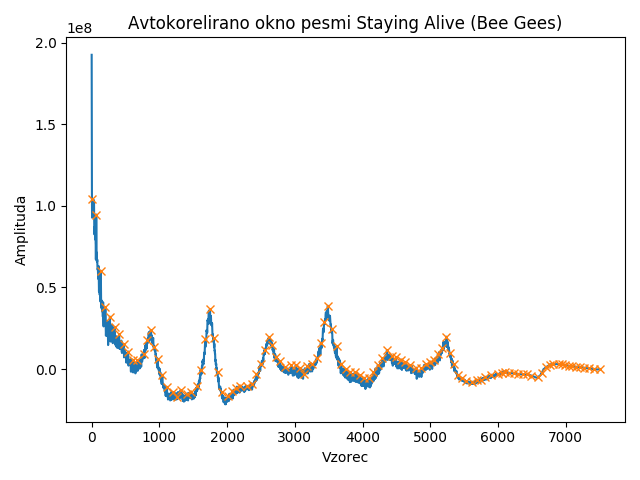
\includegraphics[scale=0.5]{images/sa_win0_dist50_peaks.png}
\caption{Avtokoreliran signal prvih 5 sekund pesmi Staying Alive (skupine Bee Gees) v modrem in vrhovi najdeni preko \textit{scipy.signal.find\_peaks} z razdaljo 50 kot oranžni križci.}
\label{peaks1}
\end{center}
\end{figure}

\begin{figure}[htbp]
\begin{center}
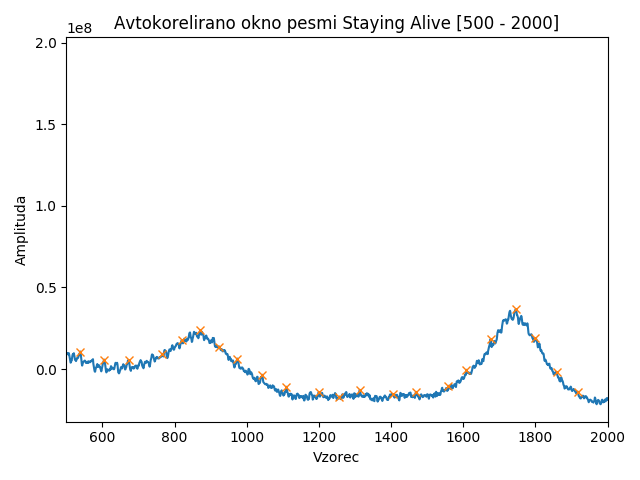
\includegraphics[scale=0.5]{images/sa_win0_dist50_peaks_zoom.png}
\caption{Približan avtokoreliran signal slike~\ref{peaks1}.}
\label{peaks1_zoom}
\end{center}
\end{figure}

\begin{figure}[htbp]
\begin{center}
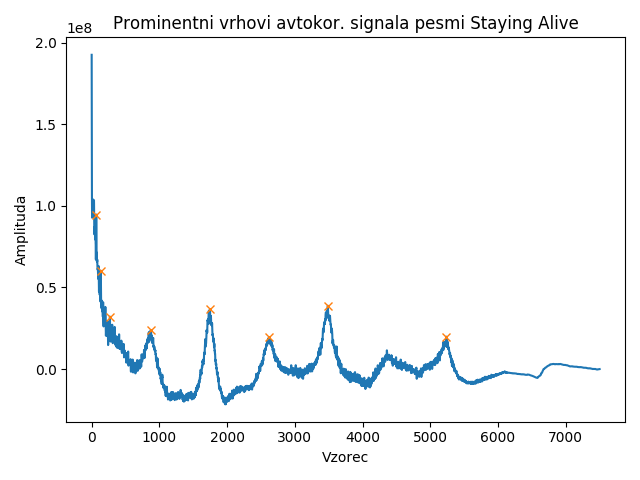
\includegraphics[scale=0.5]{images/sa_win0_dist50_peaks_prom8.png}
\caption{Vrhovi avtokoreliranega signala pesmi Staying Alive (skupina Bee Gees), najdeni s \textit{scipy.signal.find\_peaks}, pri čemer je $distance = 50$, nato pa so še sortirani preko prominence (\textit{scipy.signal.peak\_prominences}, pri čemer je $wlen = 300$. Izbranih je 8 (uporabniški parameter programa) vrhov.}
\label{peaks1_prom}
\end{center}
\end{figure}

V nadaljevanju iskanja rešitve sem se opiral na naslednjo enačbo:
\begin{equation} \label{eq:bpm}
BPM = \frac{60 \cdot F_s}{i_{sample} \cdot dec}
\end{equation}
Pri čemer je $F_s$ frekvenca vzorčenja, $i_{sample}$ je indeks vzorca, $dec$ pa predstavlja faktor podvzorčenja. S to enačbo sem pretvoril vsak vrh v ustrezen BPM, nato pa še poračunal povprečje (za boljše rezultate se je izkazala mediana) za posamezno okno. Pri uporabi 3 vrhov (kot so navedli v članku~\cite{tzanetakis2002musical}) in prej omenjenega postopka dobimo za pesem Staying Alive skupine Bee Gees BPM prikazan na sliki~\ref{bpm_sa1}. Rezultat postopka je 103.45 BPM, kar je dokaj skladno z rezultati drugih algoritmov na spletu kot tudi z namigom v navodilih. Na grafu pa so vidne tudi prve težave mojega prvotnega algoritma - nenadni poskoki, za kar je po mojem mnjenju krivo iskanje vrhov katere uporabim za preračunavanje BPM. Težave prvotnega algoritma potrdi tudi uporaba na drugih zvočnih posnetkih. Za še en kontrolni zvočni signal sem na spletu našel zvok s konstantnim ritmom 100 udarcev na minuto\footnote{Najdeno na Youtube, 100 BPM - Metronome: \url{https://youtu.be/6oz0ivczNSY}}. Z uporabo enakih parametrov kot pri pesmi Staying Alive je tukaj preračunan ritem 49 BPM, z uporabo drugih parametrov (slika~\ref{bpm_100}) pa sicer dobimo boljši rezultat vendar še vedno opazimo precej veliko nihanje.

\begin{figure}[htbp]
\begin{center}
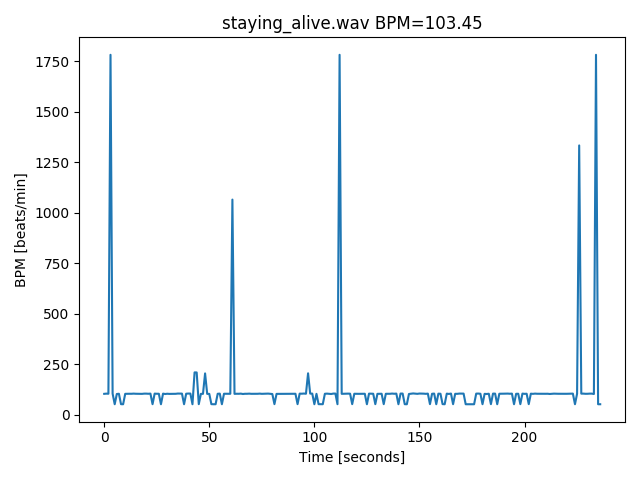
\includegraphics[scale=0.5]{images/sa_bpm_p3_orig.png}
\caption{Graf udarcev na minuto pesmi Staying Alive z uporabo prvotnega algoritma, pri čemer uporabimo 3 vrhove, $distance = 50$, in prominenco katere $wlen = 300$.}
\label{bpm_sa1}
\end{center}
\end{figure}

\begin{figure}[htbp]
\begin{center}
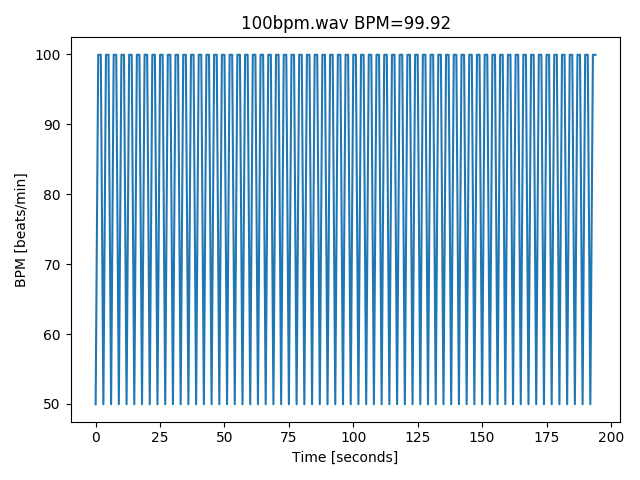
\includegraphics[scale=0.5]{images/100_bpm_orig_wlen50.png}
\caption{Graf udarcev na minuto zvočnega posnetka s konstantnim ritmom 100 BPM (težava prvotnega algoritma). Za izračun BPM so uporabljeni 3 vrhovi na okno, $distance = 50$, in prominenco katere $wlen = 50$.}
\label{bpm_100}
\end{center}
\end{figure}

\subsection{Algoritem omejenega območja}

Težavo algoritma opisanega v prejšnjem poglavju sem rešil tako, da sem omejil območje iskanja vrhov. V članku omenjajo, da si ustvarijo histogram, v katerega nato uvrščajo 3 vrhove in iz tega izračunajo povprečen BPM. Slednjega sicer pridobijo z izboljšano avtokorelacijo (skaliranje in seštevanje avtokorelacije signala pri različnih faktorjih), sam pa za izračun še vedno uporabljam enačbo~\ref{eq:bpm}. Iz enačbe ven lahko izpeljemo najnižji in najvišji indeks vzorca glede na območje udarcev na minuto (kot v članku sem vzel od 40 do 200 udarcev na minuto):
\begin{equation} \label{eq:mini}
min_{i} = \frac{60 \cdot F_s}{40 \cdot dec}
\end{equation}

\begin{equation} \label{eq:maxi}
max_{i} = \frac{60 \cdot F_s}{200 \cdot dec}
\end{equation}
S slednjima mejama pa lahko uvedemo meje v avtokoreliran signal in nato iščemo vrhove (slika~\ref{sa_peaks_new}). Z omejitvijo območja se izognemo skoraj vedno deketiranem vrhu v bližini 0 (avtokorelacija) in pa tudi ponovitvam (ni potrebno računati razlik med vrhovi). Slabost pa je, da lahko detektiramo le na območju določenim z enačbama~\ref{eq:mini} in~\ref{eq:maxi}. Poskusi kažejo, da opisani postopek deluje najbolje v primeru, ko nad omejenim območjem vzamemo le 1 vrh in sicer tistega z najvišjo vrednostjo. V kolikor vpeljemo več vrhov je potrebno dodatno spremeniti še ostale parametre (recimo dolžino okna), da dobimo podoben rezultat (glej sliki~\ref{sa_bpm_1} in~\ref{sa_bpm_10}).

\begin{figure}[htbp]
\begin{center}
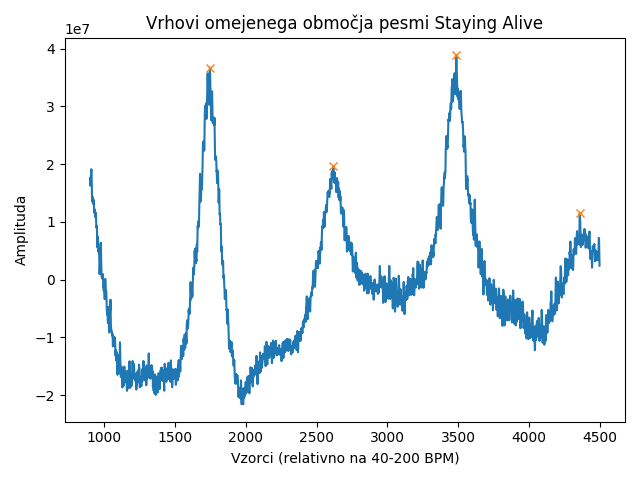
\includegraphics[scale=0.5]{images/sa_win0_dist5_prom4_new.png}
\caption{4 najbolj prominentni vrhovi na omejenem območju (900 - 4500 vzorec) prvih 5 sekund pesmi Staying Alive, razdalja med vrhovi (\textit{find\_peaks distance}) je 5.}
\label{sa_peaks_new}
\end{center}
\end{figure}

\begin{figure}
\centering
\begin{subfigure}{0.48\textwidth}
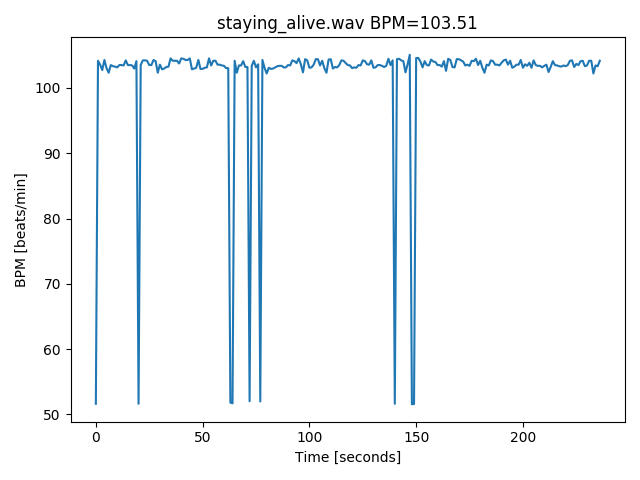
\includegraphics[width=\linewidth]{images/sa_bpm_p1_new.png}
\caption{BPM pesmi Staying Alive skozi čas, pri čemer uporabimo 1 vrh in dolžino okna 5 sekund. Uporabljen je izboljšan algoritem, kjer smo omejili območje iskanja BPM.} \label{sa_bpm_1}
\end{subfigure}
\hspace*{\fill} % separation between the subfigures
\begin{subfigure}{0.48\textwidth}
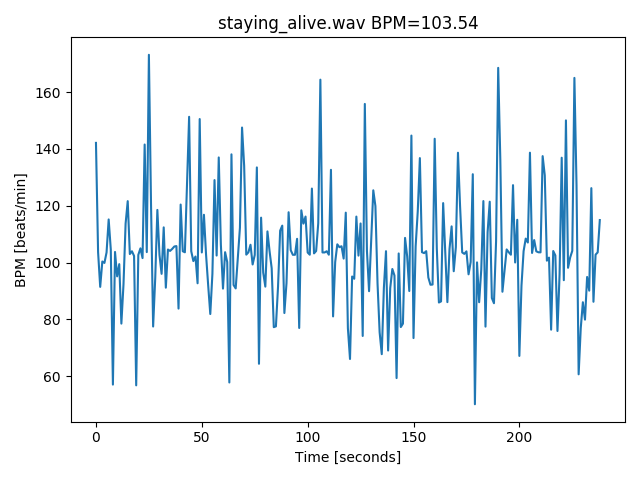
\includegraphics[width=\linewidth]{images/sa_bpm_p10_w3_new.png}
\caption{BPM pesmi Staying Alive skozi čas, pri čemer uporabimo 10 vrhov in dolžino okna 3 sekunde. Uporabljen je izboljšan algoritem, kjer smo omejili območje iskanja BPM.} \label{sa_bpm_10}
\end{subfigure}

\caption{Primerjava enega vrhova in uporabo večih. Slednje zahteva spremembo še ostalih parametrov za primerljive rezultate.} \label{sa_bpm_peak_cmp}
\end{figure}

\subsection{Testiranje na zvočnih posnetkih}

Poleg prej omenjenih parametrov sem preveril tudi uporabo povprečja in mediane za računanje BPM. Izkazalo se je, da mediana daje v mojem primeru boljše rezultate (razni poskoki na grafih se manj upoštevajo), prav tako pa sem preveril tudi ali dobimo boljše rezultate s sestavljanjem dekompoziranih signalov (in ustrezno podvzorčenje na vsaki stopnji). Povprečen rezultat udarcev na minuto se ni spremenil, po mojem mnenju pa se je polepšal prikaz BPM na grafu. Na sliki~\ref{sa_bpm_cmp} in ustreznih podslikah vidimo primerjavo uporabe podvzorčenja in samo aproksimacije ali vseh stopenj DVT. Medtem ko je na končni rezultat vpliv minimalen, se iz vidika grafa lepše opazi konstanost ritma Staying Alive v primerih, ko uporabimo sestavljen dekompoziran signal.

\begin{figure}
\centering
\begin{subfigure}{0.48\textwidth}
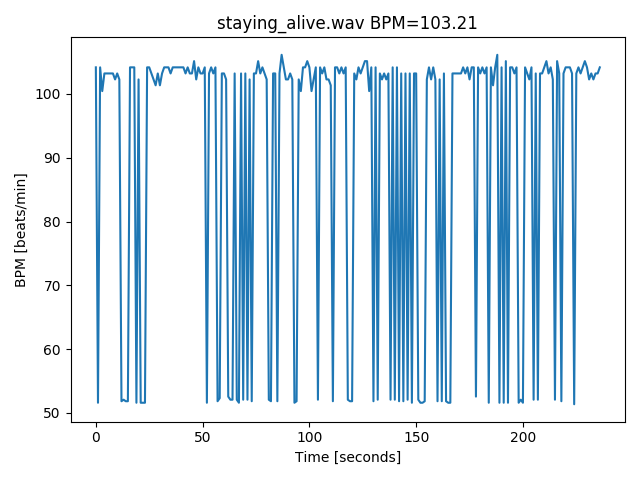
\includegraphics[width=\linewidth]{images/sa_bpm_single.png}
\caption{Kot podatke o pesmi vzamemo le aproksimacijo signala na 4. stopnji DVT. Signal tudi podvzorčimo s stopnjo 16.} \label{sa_bpm:1a}
\end{subfigure}
\hspace*{\fill} % separation between the subfigures
\begin{subfigure}{0.48\textwidth}
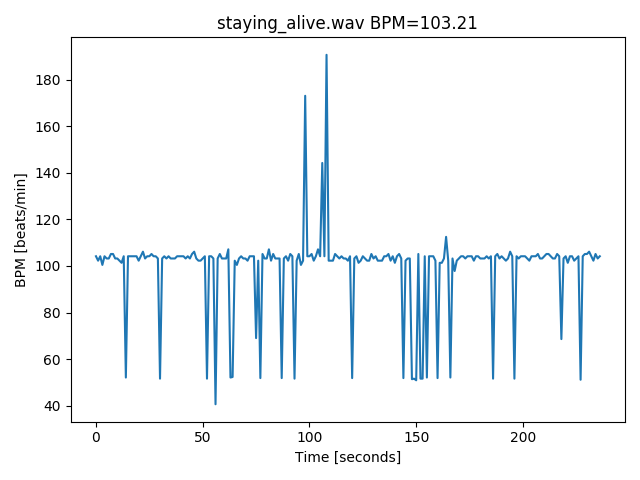
\includegraphics[width=\linewidth]{images/sa_bpm_multiple_subs16.png}
\caption{Ovojnice nad posameznimi stopnjami DVT se (ustrezno) podvzorčene združijo in podvzorčijo s faktorjem 16.} \label{sa_bpm:1b}
\end{subfigure}

\begin{subfigure}{0.48\textwidth}
\centering
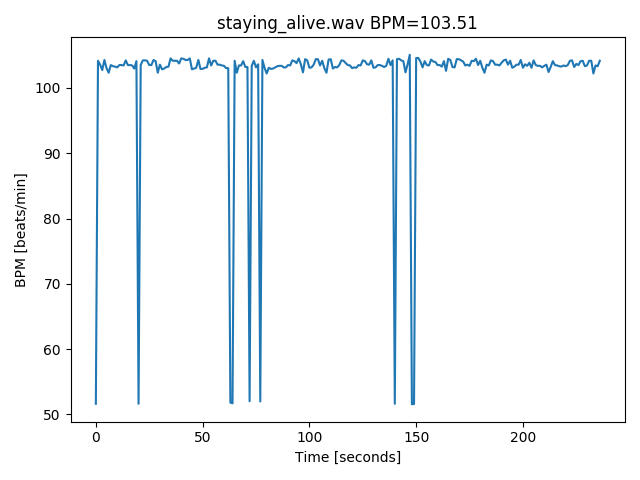
\includegraphics[width=\linewidth]{images/sa_bpm_multiple_nosubs.png}
\caption{Ovojnice nad posameznimi stopnjami le združimo (podvzorčimo glede na vsako stopnjo) brez dodatnega podvzorčenja na najnižjem nivoju.} \label{sa_bpm:1c}
\end{subfigure}

\caption{Primerjava uporabe samo aproksimacije DVT (\ref{sa_bpm:1a}), združevanje posameznih stopenj in vpeljava podvzorčenja s faktorjem (\ref{sa_bpm:1b}) in združevanje stopenj DVT brez podvzorčenja na najnižjem nivoju (\ref{sa_bpm:1c}). Uporabljena pesem je Staying Alive, pri čemer se ostali parametri razen omenjenih niso spreminjali.} \label{sa_bpm_cmp}
\end{figure}


Poleg pesmi Staying Alive in konstantnega ritma 100 BPM sem s svojim algoritmom testiral tudi druge pesmi. Rezultati\footnote{Vir za vrednosti v stolpcu BPM v tabeli~\ref{tab:rezultati} je spletna stran \url{https://songbpm.com/}} so prikazani v tabeli~\ref{tab:rezultati}.

\begin{table}[!htpb]
\centering
\renewcommand{\arraystretch}{1.5}
 \begin{tabular}{||c c c c||} 
 \hline
 Pesem & BPM & bpm.py & graf \\ [0.5ex]
 \hline \hline
 Staying Alive & 104 & {\Large 103.21} & \ref{sa_bpm:1b} \\
 Bad Guy & 135 & {\Large 135.54 } & \ref{bpm_bag_guy} \\
 Miracle & 100 & {\Large 101.35} & \ref{bpm_miracle} \\
 Bohemian Rhapsody & 143 & {\Large 144.23} & \ref{bpm_bohrhap} \\
 Lutka & 160 & {\Large 127.12} & \ref{bpm_lutka} \\
 Kažu & 170 & {\Large 160.71} & \ref{bpm_kazu} \\
 \hline
 
\end{tabular}
\caption{\label{tab:rezultati}Primerjava točnosti BPM za različne pesmi.}
\end{table}

\begin{figure}[htpb]
\begin{center}
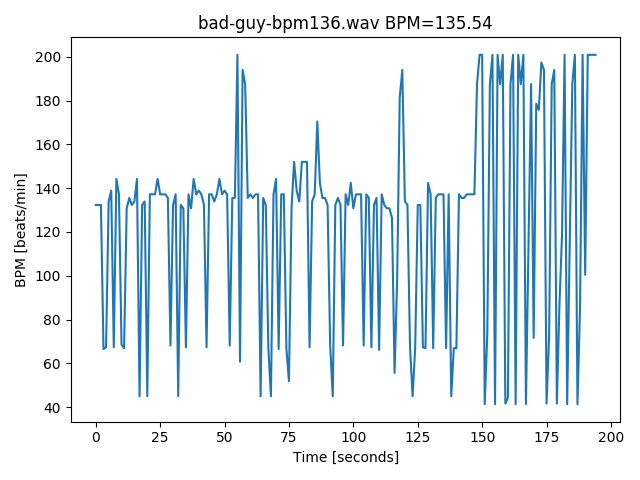
\includegraphics[scale=0.6]{images/bg_bpm.png}
\caption{BPM Graf pesmi Billie Eillish - Bad guy (\url{https://youtu.be/Jqi4GBxmwgg}).}
\label{bpm_bag_guy}
\end{center}
\end{figure}

\begin{figure}[htpb]
\begin{center}
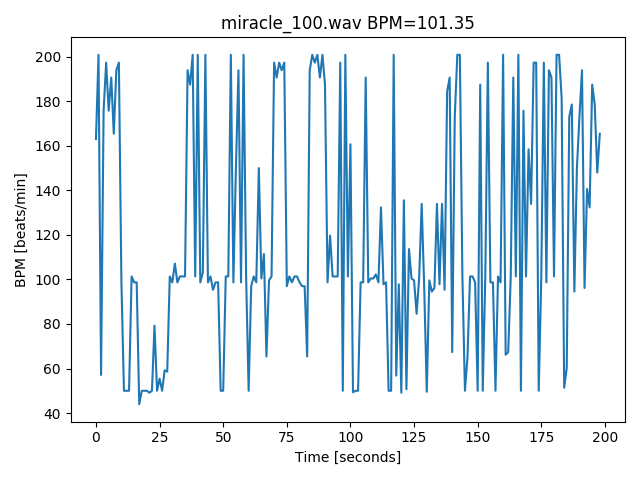
\includegraphics[scale=0.6]{images/miracle_bpm.png}
\caption{BPM Graf pesmi Caravan Palace - Miracle (\url{https://youtu.be/QdabIfmcqSQ).}}
\label{bpm_miracle}
\end{center}
\end{figure}

\begin{figure}[htpb]
\begin{center}
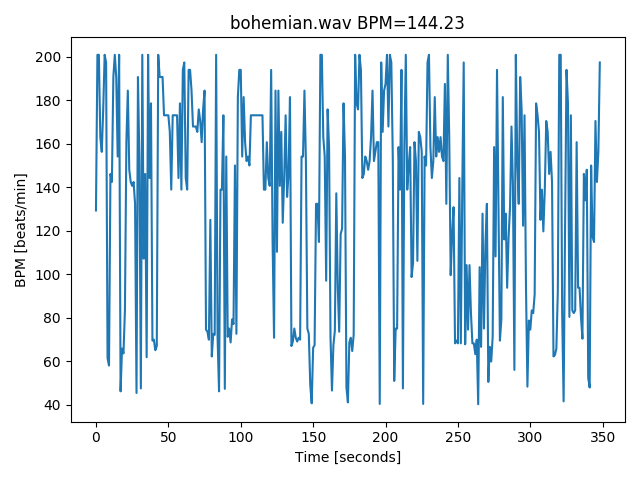
\includegraphics[scale=0.6]{images/bohemian_bpm.png}
\caption{BPM Graf pesmi Queen - Bohemian Rhapsody (\url{https://youtu.be/V8QqZ0Qb3U8).}}
\label{bpm_bohrhap}
\end{center}
\end{figure}

\begin{figure}[htpb]
\begin{center}
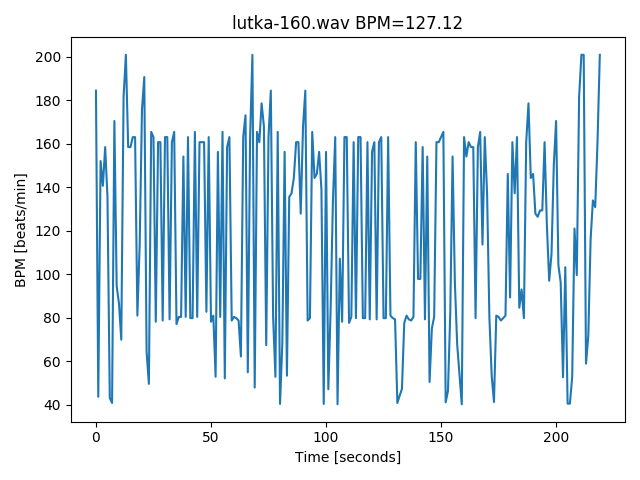
\includegraphics[scale=0.6]{images/lutka_bpm.png}
\caption{BPM Graf pesmi S.A.R.S. - Lutka (\url{https://youtu.be/E8Ms56gX-Tc}).}
\label{bpm_lutka}
\end{center}
\end{figure}


\begin{figure}[htpb]
\begin{center}
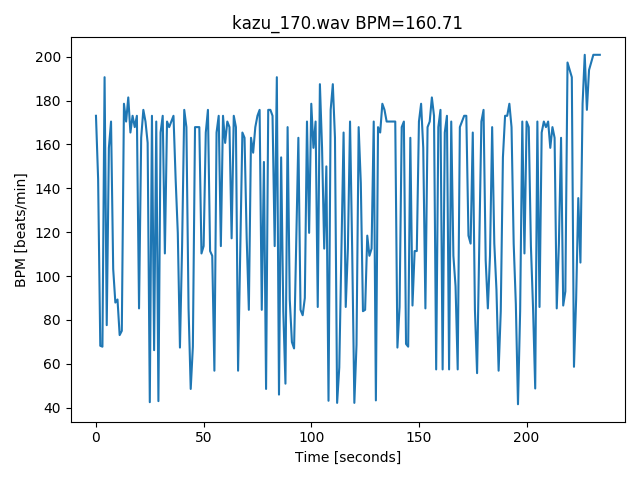
\includegraphics[scale=0.6]{images/kazu_bpm.png}
\caption{BPM Graf pesmi Dubioza Kolektiv - Kažu (\url{https://youtu.be/FZZJeMKJV3M}).}
\label{bpm_kazu}
\end{center}
\end{figure}


\bibliographystyle{plain}
\bibliography{literatura}{}

\end{document}
